%% Description: 
%%
%%

\section {Server Functionality}
\thispagestyle{plain}

The PyOPC framework also enables easy and rapid creation of OPC XML-DA
compliant servers. Implementing OPC servers is more complicated than
creating clients, however PyOPC introduces several concepts that
should greatly reduce the effort.

Most often, an OPC server will retrieve data from underlying devices
or networks, such as fieldbuses. Most of these underlying technologies
will also provide operations similar to OPC operations, such as
reading and writing. In such a situation, the OPC XML-DA server will
be similar to a proxy, which retrieves data on one side from
fieldbuses or devices, reformats it and provides it to clients on the
other side, such as depicted in figure \ref{opc_proxy}.

\begin{figure}[ht]
\htmlborder{1}
\centering
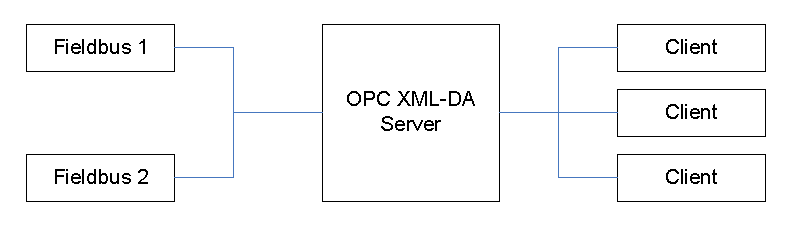
\includegraphics[scale=0.7]{graphics/opc_proxy.eps}
\caption{OPC XML-DA Server as a Proxy}
\label {opc_proxy} 
\end{figure}

PyOPC introduces a server class, the {\sl XDAServer}, which provides
methods for each OPC operation. This class can be inherited and the
methods can be overridden by custom implementations, as illustrated
in figure \ref{server_hierarchy}.

\begin{figure}[ht]
\htmlborder{1}
\centering
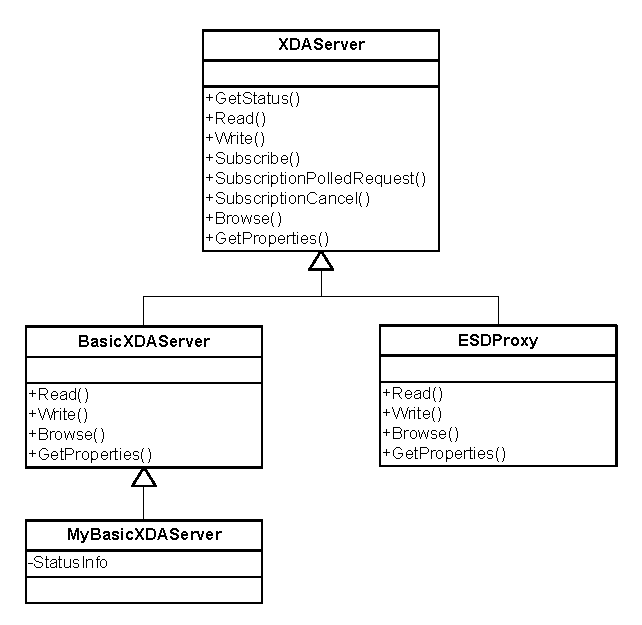
\includegraphics[scale=0.7]{graphics/server_hierarchy.eps}
\caption{Server Class Hierarchy}
\label {server_hierarchy} 
\end{figure}

For instance, the class {\sl BasicXDAServer} inherits from {\sl
XDAServer}.  The BasicXDAServer class overrides certain functionality
of its parent class, such as Read and Write, where it implements its
own functionality. However, this is still a quite general class and
is not intended for the actual server instance. Instead, another class,
{\sl MyBasicXDAServer} inherits from the class, which defines various
attributes that define the runtime parameters for the server instance,
such as ``GetStatus'', which may be set to any custom value.

This way, implementing a OPC XML-DA server with PyOPC leads to a three-level
class hierarchy:

\begin{enumerate}
\item The basic XDAServer class that implements general functionality, which
is provided by the PyOPC framework
\item A server-specific class that overrides certain operations to
implement its custom functionality, which has to be implemented for
the dedicated system
\item The production-specific class, which defines several production 
specific parameters and is used for the server instance.
\end{enumerate}

Listing \ref{ex_simple_server} shows the code for a very basic server
that inherits from the BasicXDAServer class, which enables to define
several OPC items in the server instance itself. These OPC items can
then be read and written by OPC clients.

\lstset{language=C}
\begin{lstlisting}[caption={Simple OPC XML-DA Server}
                   ,label=ex_simple_server] 
import random
from twisted.internet import reactor,defer
from PyOPC.servers.basic import BasicXDAServer

# Read sample OPC items for testing
import sample_items

class MyXDAServer(BasicXDAServer):
    OPCItems = sample_items.TestOPCItems
    StatusInfo = 'My Basic OPC XML-DA Server'

    def GetStatus(self, (IPH,inOptions,outOptions)):
        ''' Custom GetStatus that alters the Product Version'''

        outOptions['ProductVersion'] = str(random.choice(range(1,10)))
        
        return super(MyXDAServer, self).GetStatus((IPH,inOptions,outOptions))
\end{lstlisting}

In line 9 some predefined OPC items are set in the server instance. These
items are defined in an external module, which is imported in line 6.
Moreover the MyXDAServer class defines the class attribute ``StatusInfo''
which will then be used in the OPC ``GetStatus'' operation.

Line 12-18 shows how the ``GetStatus'' operation is overridden by the
inherited class. In this method, the OPC option ``Product Version'' is
set to an arbitrary number between 1 and 9.

Line 17 is very important: this line calls the method of the parent
class and returns the results. Python does not automatically call its
parent class, this has to be done manually.  However, it is mandatory
in PyOPC that an overridden OPC operation has to call the method in
its parent class. The reason is that this parent method fulfills
several needed functionality, such as setting several other needed OPC
options to maintain compatibility with the OPC XML-DA specification.
The call of the superclass method has always to be done at the
end of the custom method.

The above listing also shows how data such as the global options and
the OPC items are passed. It is obvious that any XDAServer-based
method, which represents an OPC operation, has to process parameters
from the client request message and has to create several appropriate
output parameters, which form the base of the response message. In
PyOPC, these request and response parameters are passed from one
method to another and thus also from each child to its parent method,
such as shown in figure \ref{opc_parameters}.

\begin{figure}[ht]
\htmlborder{1}
\centering
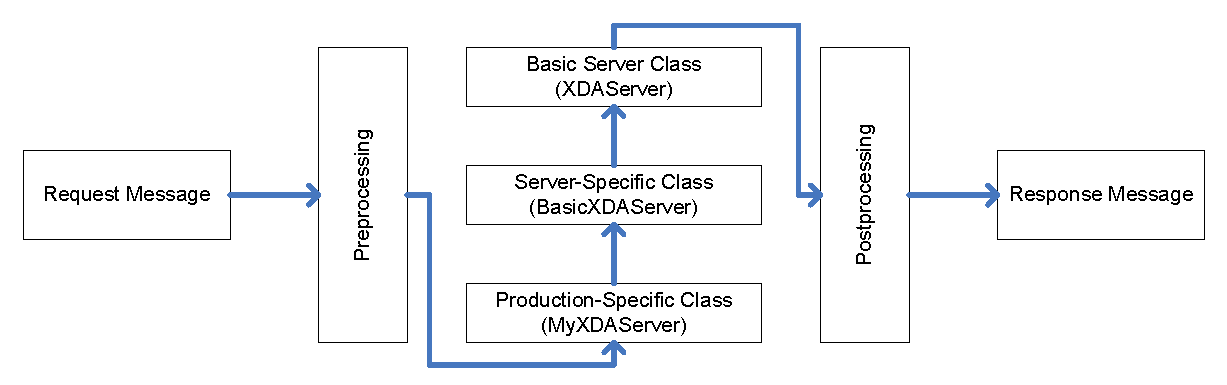
\includegraphics[scale=0.7]{graphics/opc_parameters.eps}
\caption{OPC Parameter Passing}
\label {opc_parameters} 
\end{figure}

Similar to the PyOPC-based client, the request and response messages
are represented by a Python dictionary that contains the global OPC
options and a list of ItemContainer objects, representing the OPC
items. It can be observed in figure \ref{opc_parameters} that 
OPC data is passed from one method to another. All these methods
require the input parameters and will set or alter certain output
parameters.

Therefore it is appropriate to aggregate the input and output
parameters in one Python object, which is then passed from one method
to another. Therefore each PyOPC method, which represents an OPC
operation, must define a Python tuple as a parameter which contains
the following three objects:

\begin{enumerate}
\item The {\bf Item Pair Holder} (IPH), a special object that contains
an input and output list of ItemContainer objects. These lists have
always to be of the same length and every input ItemContainer object
has a corresponding output ItemContainer object. These internal
ItemContainer lists are normally not directly accessed. Instead, the
ItemPairHolder object implements an ``append'' method, which can be
used to append an input and output ItemContainer object. Moreover the
object is iterable, which is most often needed by OPC operation
methods.

Listing \ref{ex_IPH} shows how such an ItemPairHolder can be created
and managed:

\lstset{language=C}
\begin{lstlisting}[caption={Creating and Managing the ItemPairHolder object}
                   ,label=ex_IPH] 
IPH = ItemPairHolder()
IPH.append(inItem, outItem)
for inItem, outItem in IPH:
   outItem.ItemPath = inItem.ItemPath
\end{lstlisting}

The example listing first creates an ItemPairHolder object and appends
some predefined ItemContainer objects. Then one certain attribute of
the output item, the ``ItemPath'' is set to its corresponding input
attribute.

\item The {\bf input options} (inOptions), a Python dictionary, which
contains all global input options
\item The {\bf output options} (outOptions), a Python dictionary, which
contains all global output options
\end{enumerate}

\subsection*{Server Configuration}

The server can be configured through several class attributes. These
attributes can either be overridden in the inheriting object, or can
also be specified at the server object instantiation.

The basic {\sl XDAServer} class provides the following options. (Their
default values are given in parentheses.) Some of them are are further
described in later sections:

\begin{description}

\item[AutoItemCache {\sl (True)}:] This option enables the automatic
OPC item caching.
\item[WritePurgeCache {\sl (True)}:] Denotes if the item cache should be
flushed after an item is written. 
\item[DefaultMaxAge {\sl (1000)}:] The default maximum age of an item.
\item[BufferSize {\sl (100)}:] The default subscription buffer size in
number of items.
\item[ThreadedParsing {\sl (True)}:] One of the most CPU-intensive
tasks is the parsing of the incoming SOAP message. In order to speed
up the server, it is possible to execute the parser in a separate
thread, so that the server can execute other requests in
parallel\footnote{The speed gain is currently not very significant, as
fast XML parsers are quite efficient compared to other tasks, such as
serializing the SOAP message.}.
\item[ThreadPoolSize {\sl (5)}:] The maximum amount of concurrent
threads.
\item[SubscriptionPingRate {\sl (10000)}:] The default subscription ping
rate in milliseconds.
\item[MaxPingRate {\sl (86400000 = 1 Day)}:] The maximum ping rate that
may be specified by a client.
\item[MaxSamplingRage {\sl (100)}:] The maximum sampling rate in
milliseconds that clients may specify.
\item[HandleProperty\_value/quality/timestamp/scanRate {\sl (True)}:]
Denotes if the above properties are automatically generated/handled.
\end{description}

\subsection{Preprocessing and Postprocessing}

The PyOPC XDAServer class automatically parses incoming SOAP messages
and creates appropriate PyOPC objects, which represent the incoming
message. After that, the preprocessing stage prepares and handles some
of the following options of the outgoing message:

\begin{description}

\item[RcvTime:] This option is set to the time, the SOAP message was
received by the server.
\item[ClientRequestHandle:] The content of the incoming
ClientRequestHandle is automatically copied to the outgoing message.
\item[RevisedLocaleID:] If the requested locale is not available, the
server automatically chooses the first available locale and returns it
with this options.
\item[ServerState:] This option is set to the ServerState attribute of
the server class, the default is ``running''.

\end{description}

After this stage, the server operation methods are executed.
Therefore the data from the preprocessing stage is available in these
methods and may be modified.  For instance, the read operation may
check for the option ``RevisedLocaleID'' in the outgoing message and
set it to a different locale.

After the server operations are finished, the PyOPC objects, which
represent the incoming and outgoing SOAP messages is handed over to
the postprocessing stage, which handles and modifies the following
options:

\begin{description}

\item[Unhandled Items:] As denoted above, the incoming and outgoing
OPC items are stored in the ItemPairHolder object. The preprocessing
stage will create this object, which contains an incoming
ItemContainer object and an associated, empty outgoing ItemContainer
object. The operations should then fill this outgoing item with
appropriate data. If, however, the outgoing ItemContainer object is
still empty\footnote{A ContainerItem is empty, if the attribute
'IsEmpty' is set to true. This happens if it is created such as
i=ItemContainer() and no attribute is ever set.} in the postprocessing
stage, an error of the type ``PYO\_E\_EMPTYITEM'' is associated with
it, denoting that the item contains no data.

\item[ErrorText:] If {\sl ReturnErrorText} is set to false in the
request message, any error text in the outgoing message is
deleted. Otherwise the error text will be kept, and if there is none
in the outgoing message, it will be set to a blank string.
\item[DiagnosticInfo:] If {\sl ReturnDiagnosticInfo} is set to false
or is omitted in the request message, any diagnostic info in the
outgoing message is deleted. Otherwise the diagnostic info will be
kept, and if there is none in the outgoing message, it will be set to
a blank string.
\item[Timestamp:] If {\sl ReturnItemTime} is set to false or is
omitted in the request message, any item-related timestamp in the
outgoing message is deleted. Otherwise the timestamp will be kept,
and if there is none in the outgoing message, it will be set to 
the current time.
\item[ItemPath/ItemName:] If {\sl ReturnItemPath/Name} is set to false
or is omitted in the request message, any ItemPath/Name in the
outgoing message is deleted. Otherwise the ItemPath/Name will be kept,
and if there is none in the outgoing message, it will be set to a
blank string.
\item[ClientItemHandle:] The ClientItemHandle of each incoming item is
copied to the according outgoing item.
\item[ReplyTime:] The ReplyTime in the outgoing message is set to the
current time, unless it has not been already set a previous server
method.

\end{description}

\subsection{Item Caching and Subscriptions}

PyOPC provides support for advanced OPC XML-DA services, such as 
subscriptions and Item Caching. Unless these services are disabled,
they are automatically available at any PyOPC-based OPC server.

\subsubsection*{Item Caching}

OPC XML-DA servers normally retrieve data from underlying systems,
such as fieldbuses. Different client will then access these items
through the OPC server. There may be situations, where many clients
access the same OPC item over and over. These client requests will
therefore lead to a significant load on underlying systems and may
even exceed their capabilities.

One solution to this problem is caching: when the OPC server retrieves
an item from an underlying system, it stores it for a predefined amount
of time. These cached items are then available for OPC clients, therefore
client requests do not necessarily lead to data retrieval from underlying
systems.

In the client request message, the option ``MaxAge'' may be specified,
denoting how old the item may be. If MaxAge is greater than the time
the item is cached, the server will build the response message upon
the cached item, otherwise the server will retrieve new data.

The PyOPC framework does automatically implement OPC item caching, if
the server attribute ``AutoItemCache'' is set to true (which it is by
default). The developer can also specify the attribute
``DefaultMaxAge'', which defines the maximum age in milliseconds for
requests that do not provide the MaxAge option.

The exact item caching mechanism is illustrated in figure
\ref{item_caching}:

\begin{figure}[ht]
\htmlborder{1}
\centering
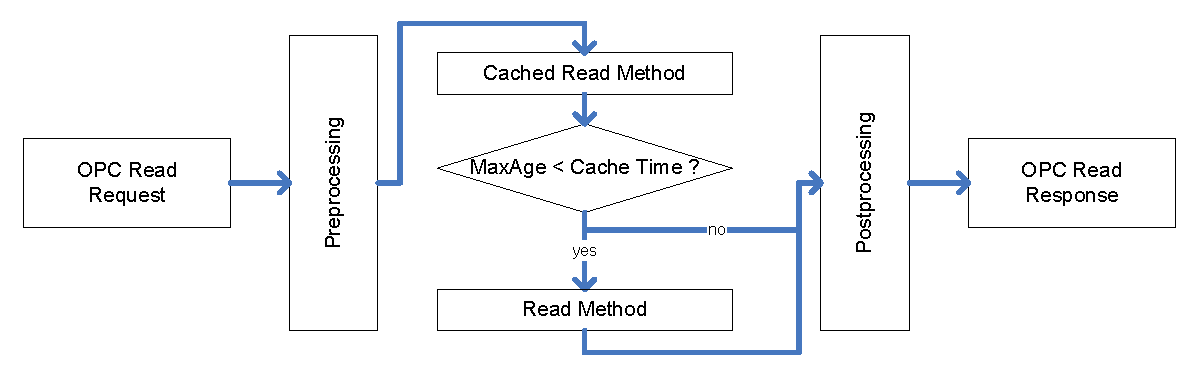
\includegraphics[scale=0.7]{graphics/item_caching.eps}
\caption{Mechanism of PyOPC Item Caching}
\label {item_caching} 
\end{figure}

If an OPC Read request message is received by the server and ``AutoItemCache''
is set to true, the XDAServer method ``CachedRead'' is called. This method
decides whether to return cached data regarding the MaxAge parameter or
whether it calls the server's read method, which retrieves the data from
the underlying system.

This way, the developer does not need to regard item caching, he has
to code only the data retrieval itself. His read method will be only called
if the maximum allowed age is smaller than the time, the item is cached.

Write operations update data in underlying devices. Therefore by
default the read cache of a written item is flushed. However, in
certain situations it may be appropriate not to clear the
cache. Therefore PyOPC provides the option ``WritePurgeCache'' which
can be set to false to omit the automatic cache flushing.

\subsubsection*{Subscriptions}

In order to observe OPC items, one could theoretically periodically
poll OPC items with read operations and check for changes. However,
such polling leads to an unnecessary network and server
load. Therefore \cite{OPCXMLDA} introduces so-called ``subscriptions''
and specifies three related OPC operations.

OPC clients may subscribe to items, which basically commands the
server to observe these items for changes. Such changes will be stored
by the server and can later be retrieved by the client.

Implementing such a subscription mechanism in the server is quite
complicated. The OPC XML-DA specification describes several complex
issues, such as deadband (recording items only if they exceeded a
predefined value) and the so-called extended subscription
architecture. A detailed description of these topics is given in
\cite{OPCXMLDA}.

To ease the development of OPC XML-DA servers, the PyOPC framework
implements a default mechanism for subscriptions which is
automatically available and functional for all OPC XML-DA servers
based on the {\sl XDAServer} class. The basic idea is that most
underlying systems such as fieldbuses have a read operation that is
roughly similar between different systems, while system notifications
- a common way to observe datapoints for changes - can be very
different on fieldbus systems. Therefore the most compatible way is to
utilize the read operation for subscriptions.

Therefore developers only have to implement the read operation and will
thus automatically enable subscriptions. The basic mechanism is illustrated
in figure \ref{pyopc_subs}.

\begin{figure}[ht]
\htmlborder{1}
\centering
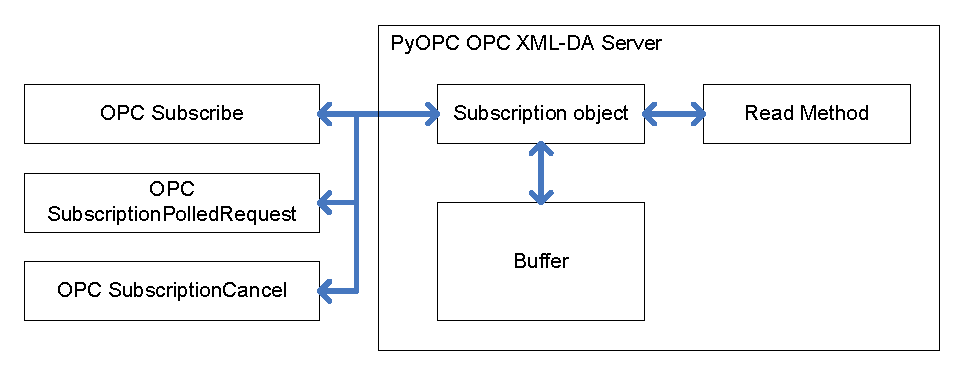
\includegraphics[scale=0.7]{graphics/pyopc_subs.eps}
\caption{Subscriptions in PyOPC}
\label {pyopc_subs} 
\end{figure}

It can be seen that a client can utilize the following three
operations to handle subscriptions:

\begin{itemize}
\item {\sl Subscribe} creates a subscription object in the server.
This subscription object will then utilize the server's read operation
to periodically poll the underlying system for changed items. These
changed items are then stored - either in the subscription object
itself, or, if specified by the client, in a subscription buffer,
which is shared among all subscriptions.
\item {\sl SubscriptionPolledRequest (SPR)} is then used by clients
to retrieve all changed values.
\item {\sl SubscriptionCancel} can then be used to cancel the subscription
which results in the deletion of the subscription object.
\end{itemize}

PyOPC also covers all complex subscription-related issues, such as the
PingRate, HoldTime/WaitTime, deadband and more, therefore developers
do not have to deal with these issues.

The following functionality can be configured in the server object:

\begin{description}
\item[BufferSize:] All OPC subscriptions share one buffer, which is
used to store changed items until they are fetched by the client via
the SPR operation. With the BufferSize attribute, the number of items
can be specified that the buffer can hold. If more items than this
number are stored in the buffer, the oldest entries are lost.
\item[SubscriptionPingRate:] If the client did not specify a ping
rate, this predefined value will be used. The ping rate defines, how
much time may elapse between two client polls. If the ping rate is
exceeded, the subscription is automatically canceled.
\item[MaxPingRate:] This is the maximum ping rate, a client may specify.
\item[MaxSamplingRate:] As denoted above, the subscription object
periodically fetches (samples) item values from underlying devices.
This sampling can be very demanding for the underlying system,
therefore a maximum sampling rate can be specified in the server. If a
client requests a higher sampling rate than this value, it is revised
to this value by the server.

OPC server developers should set this to a suitable value: the maximum
sampling rate should never be higher than the time that is needed for
a read request.
\end{description}

It should be denoted that PyOPC allows only one SPR for one
subscription object at a time. If a second concurrent SPR is issued,
the server will return an error\footnote{The OPC XML-DA specification
is quite loose on this topic, therefore in PyOPC concurrent SPRs are
prohibited.}.

An OPC server developer may also implement his own subscription
mechanisms. This can be done by overriding the three XDAServer methods
{\sl Subscribe, SubscriptionPolledRequest} and {\sl
SubscriptionCancel}, however, this will most often not be necessary.

\subsection{Operation Specific Functionality and Other Issues}

\subsubsection*{Automatic Readback}

In OPC write requests, the client may specify the option
``ReturnValuesOnReply''. If this option is set to true, the server
will read back the written values. This is accomplished by
calling the servers read method.

\subsubsection*{Browsing}

Clients may specify OPC properties in a browse request, which will
then be returned along with the appropriate browse result. In order to
retrieve these properties, the server's Browse method will call the
servers GetProperties method.

\subsubsection*{Property Handling}

Certain OPC properties, namely {\sl value, quality, timestamp} and
{\sl scanRate} can be automatically handled by the PyOPC
framework. This way, these four properties will be automatically
available for all OPC items.

The values of these properties will be retrieved as follows:

\begin{itemize}
\item The values of the {\sl value, quality} and {\sl timestamp} 
properties are simply retrieved with the servers read method,
which contains all needed data.
\item The value of {\sl scanRate} is set to MaxSamplingRate.
\end{itemize}

\subsubsection*{Logging}

PyOPC based servers also support detailed logging and provides the
following three different logs:

\begin{description}
\item[Access Logging:] If a client accesses the PyOPC server, the
clients IP address and the requested SOAPAction, which defines
the OPC operation is logged in this file. The default file name
for the access log is ``access.log''.
\item[Error Logging:] PyOPC server errors are kept in this log.
Its default name is ``error.log''.
\item[Debug Information:] During development and tests, it is often
interesting for the programmer to have access to further information,
especially to the client/server communication. Therefore PyOPC logs
the SOAP messages along with the HTTP header in a pretty-printed
style. By default the debug log is disabled.
\end{description}

The file names of these logs can be configure by setting the server
attributes ``access\_log\_fn'', ``error\_log\_fn'' and
``http\_log\_fn'' to the desired name. Moreover, logging can also be
omitted by setting one or more of these attributes to a blank string.

\subsubsection*{Setting Up an OPC Server Instance}

As the server classes of PyOPC are based on the Twisted framework, it
is also utilized to set up the OPC server instance. This can be done
as shown in listing \ref{ex_start}, which implies the proper
definition of the class ``MyXDAServer'', as already shown in listing
\ref{ex_simple_server}.

\lstset{language=C}
\begin{lstlisting}[caption={Instantiating and Starting a PyOPC-based
OPC XML-DA Server}
                   ,label=ex_start] 
from twisted.web import resource, server
xdasrv = MyXDAServer(http_log_fn = 'http.log')
root = resource.Resource()
root.putChild('',xdasrv)
site = server.Site(root)
reactor.listenTCP(8000, site)
reactor.run()
\end{lstlisting}

Line 1-2 import all needed Twisted modules and create the PyOPC
server object. In line 3, a Twisted resource object is created, where
servers can be added, such as shown in line 4. Line 5-7 then starts
the server. This server will then be reachable under the address
``http://server:8000/''.

A Twisted resource.Resource object is not limited to one PyOPC server
instance, instead it is possible to add multiple server objects, such
as shown in listing \ref{ex_multiserver}, which are then reachable
under different URLs.

\lstset{language=C}
\begin{lstlisting}[caption={Adding Multiple PyOPC Server Objects to
One Twisted Resource}
                   ,label=ex_multiserver] 
root = resource.Resource()
root.putChild('srv1',MyXDAServer1())
root.putChild('srv2',MyXDAServer2())
root.putChild('srv3',MyXDAServer3())
\end{lstlisting}

\subsection{Contributed Servers}

The PyOPC framework implements two simple servers, which on the one
hand can be seen as a reference design and may on the other hand be
used for setting up simple test servers.

\subsubsection*{BasicXDAServer}

This simple server does not retrieve data from other resources,
instead the OPC item data can be directly defined in the server.

Listing \ref{ex_basicxdaserver} shows the code of a server that is
based on the BasicXDAServer class:

\lstset{language=C}
\begin{lstlisting}[caption={PyOPC server based on the class 
BasicXDAServer}
                   ,label=ex_basicxdaserver] 
class MyXDAServer(BasicXDAServer):
    OPCItems = (ItemContainer(ItemName='sample_integer',
                               Value=14,
                               QualityField='good'),
                ItemContainer(ItemName='sample_float',
                               Value=96.43,
                               QualityField='good'))
\end{lstlisting}

This server defines two OPC items, which can then be accessed
by OPC XML-DA clients.

\subsubsection*{ESDProxy}

This server can be seen as a reference design for OPC servers that
retrieve OPC data from external sources. A detailed description of
this server can be found in \cite{diplomarbeit}.